\chapter{The ATLAS Detector}

\indent The ATLAS detector (\textbf{A} \textbf{T}oroidal \textbf{L}HC \textbf{A}pparatu\textbf{S}) is one of two general purpose physics detectors designed to study the products of proton-proton collisions at the LHC. The detector is composed of a variety of specialized subsystems, designed to fully capture a wide array of physics processes. The apparatus is 25m high, 44m in length, and weighs over 7000 tons \cite{atlas_overview}. The LHC beam pipes direct proton beams to an interaction point at the center of ATLAS, and the cylindrical detector design captures a complete 360\degree\ view of the \textit{event}, tracking all particles that result from the collision.\par

\indent The main components of the ATLAS detector are the Inner Detector (ID) which provides high precision tracking of charged particles leaving the collision vertex, the calorimeter system which measures the energy of electromagnetic and hadronic objects, and the Muon Spectrometer (MS) which gives detailed information about muons that reach the outer radii of the detector. Two magnet systems, a 2 T solenoid magnet surrounding the ID, and a 0.5-1.0 T toroid magnet system situated throughout the MS, produce magnetic fields which bend the trajectory of charged particles traversing the detector. In addition to the main detector components, dedicated forward detectors monitor beam conditions and instantaneous luminosity, and an online trigger system reduces the data rate to a manageable level for storage. Each of these components will be discussed in further detail in this chapter. \par

\section{Coordinate System and Geometry}

\indent The ATLAS detector employs a right hand cylindrical coordinate system. The $z$ axis is aligned with the beam line, and the x-y plane sits perpendicular to the beam line. The coordinate system origin is centered on the detector, such that the origin corresponds with the interaction point of the two colliding beams. The detector geometry is usually characterized by polar coordinates, where the azimuthal angle $\phi$ spans the x-y plane. The polar angle $\theta$ represents the angle away from the beam line, or $z$ axis. $\theta = 0$ aligns with the positive $z$-axis, and $\phi = 0$ aligns with the positive x-axis. \par

\indent The polar coordinate $\theta$ is generally replaced by the Lorentz invariant quantity \textit{rapidity} or $y$:

\begin{equation}
	y = \frac{1}{2} ln(\frac{E+p_z}{E-p_z}) .
\end{equation}

This substitution is advantageous because objects in the detector are traveling at highly relativistic speeds. The relativistic speed also means that the masses of the particles are generally small compared to their total energy. In the limit of zero mass, the rapidity $y$ reduces to the pseudorapidity $\eta$, which can be calculated directly from the polar angle $\theta$:

\begin{equation}
	\eta = -ln(\frac{\theta}{2}) .
\end{equation}

The distance between physics objects in the detector is generally expressed in terms of the solid angle between them $\Delta R$: 

\begin{equation}
	\Delta R = \sqrt{\Delta\phi^2 + \Delta\eta^2}
\end{equation}

\par

\indent Figure \ref{fig:ATLASgeometry} depicts the orientation of the coordinate system with respect to the ATLAS detector, while Figure \ref{fig:etaTheta} illustrates the relationship between $\theta$, $\eta$, and the beamline axis $z$. Direct or ``head on" proton-proton collisions are more likely to results in objects whose momentum is directed along transverse plane (low $|\eta|$); glancing proton-proton collisions are more likely to result in objects whose momentum is directed along the $z$-axis (high $|\eta|$). Due to the difference in the nature of these collisions, as well the as the cylindrical design of the ATLAS detector, the detector is divided into regions of low and high $\eta$. Each subsystem has a ``central" or ``barrel" region covering low $|\eta|$, while the ``forward" or ``end-cap" regions cover the area up to $|\eta|$ = 4.9. Each of the three main ATLAS subsystems will be discussed in the following sections.

\begin{figure}
     \centering
     \begin{subfigure}[b]{0.45\textwidth}
         \centering
         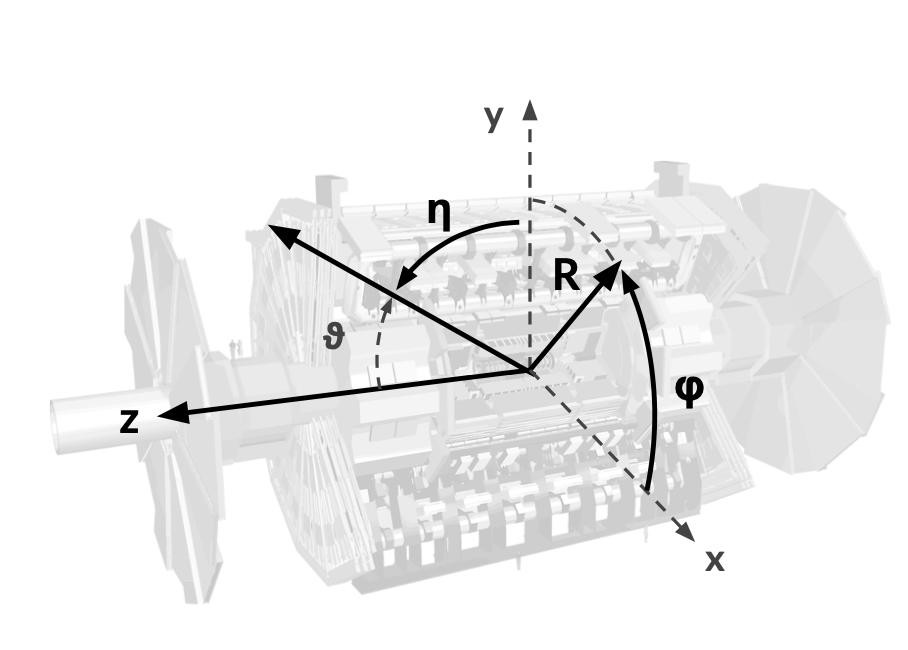
\includegraphics[width=\textwidth]{figures/ch3/ATLASgeometry.png}
         \caption{The ATLAS geometry}
         \label{fig:ATLASgeometry}
     \end{subfigure}
     \hfill
     \begin{subfigure}[b]{0.45\textwidth}
         \centering
         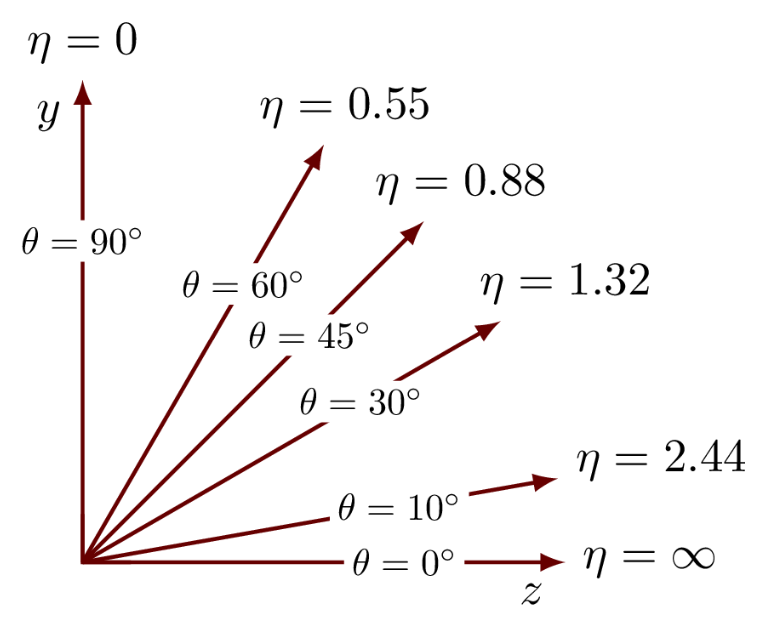
\includegraphics[width=\textwidth]{figures/ch3/etaTheta.png}
         \caption{Relationship between $\eta$ and $\theta$}
         \label{fig:etaTheta}
     \end{subfigure}
     \hfill
     \caption {ATLAS coordinate system and geometry}
\end{figure}

\section{Inner Detector}

\indent The Inner Detector (ID) is the ATLAS subsystem closest to the interaction point. The primary purpose of the ID is to determine the charge, momentum, and trajectory of charged particles passing through the detector. With this information the ID is also able to precisely determine interaction vertices. \par

\indent The ID is composed of three sub-detectors; the Pixel Detector, the Semiconductor Tracker (SCT) and the Transition Radiation Tracker (TRT). Figure \ref{fig:innerDetector} shows the location of these three subsystems with respect to each other and the interaction point. \par

\begin{figure}
        \centering
	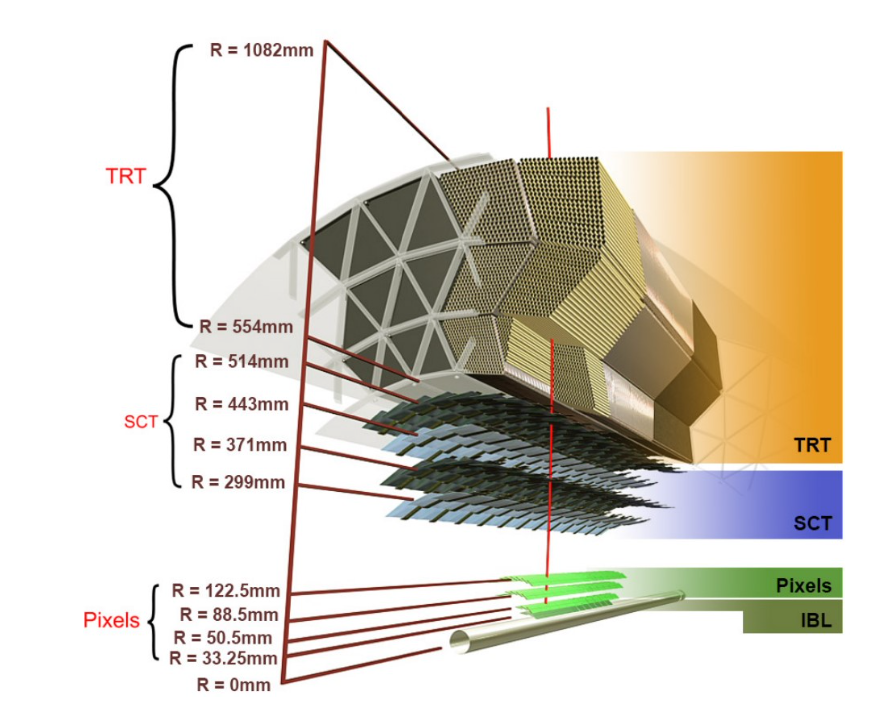
\includegraphics[width=0.6\textwidth]{figures/ch3/innerDetector.png}
	\caption{A 3D visualization of the structure of the ID in the barrel region \cite{innerDet}}
	\label{fig:innerDetector}
\end{figure}

\subsection{Pixel Detector}
The pixel detector is the first detector encountered by particles produced in LHC collisions. The original pixel detector consists of 3 barrel layers of silicon pixels, positioned at 5 cm, 9 cm and 12 cm from the beamline. There are also 3 disks on each end-cap positioned 50 - 65 cm from the interaction point, providing full coverage for $|\eta| < 2.2$. The layers are comprised of silicon pixels each measuring 50 $\times$ 400 $\mu$m$^2$, with 140 million pixels in total. The pixels are organized into modules, which each contain a set of radiation hard readout electronics chips. In 2014, the Insertable B-layer (IBL) was installed, creating a new innermost layer of the pixel detector sitting just 3.3 cm from the beamline. The pixels of the IBL measure 50 $\mu$m by 250 $\mu$m, and cover a pseudo-rapidity range up to $|\eta| < 3$. The IBL upgrade enhances the pixel detector's ability to reconstruct secondary vertices associated with short-lived particles such as the b-quark. The improved vertex identification also helped compensate for increasing pile-up in Run 2 \cite{atlas_overview}. 

\subsection{Semiconductor Tracker}
The SCT provides at least 4 additional measurements of each charged particle. It employs the same silicon technology as the Pixel Detector, but utilizes larger silicon strips which measure 80 $\mu$m by 12.4 cm. The SCT is composed of 4 barrel layers, located between 30 cm and 52 cm from the beamline, and 9 end-cap layers on each side. The SCT can distinguish tracks that are separated by at least 200 $\mu$m.

\subsection{Transition Radiation Tracker}
The TRT provides an additional 36 hits per particle track. The detector relies on gas filled straw tubes, a technology which is intrinsically radiation hard. The straws which are each 4 mm in diameter and up to 150 cm in length and filled with xenon gas. The detector is composed of about 50000 barrel region straws and 640000 end-cap straws, comprising 420000 electronic readout channels. Each channel provides a drift time measurement with a spatial resolution of 170 $\mu$m per straw. As charged particles pass through the many layers of the detector, transition radiation is emitted. The use of two different drift time thresholds allows the detector to distinguish between tracking hits and transition radiation hits. 

\section{Calorimeters}
The ATLAS calorimeter system is responsible for measuring the energy of electromagnetically interacting and hadronically interacting particles passing through the detector. The calorimeters are located just outside the central solenoid magnet, which encloses the inner detectors. The calorimeters also stop most known particles, which the exception of muons and neutrinos, preventing them from traveling to the outermost layers of the detector. The ATLAS calorimetry system is composed of two subsystems - the Liquid Argon (LAr) calorimeter for electromagnetic calorimetry and the Tile calorimeter for hadronic calorimetry. The full calorimetry system is shown in Figure \ref{fig:calorimeters}.

\begin{figure}
        \centering
	\includegraphics[width=0.7\textwidth]{figures/ch3/calorimeter.png}
	\caption{ATLAS calorimetery system \cite{calorimeter_img}}
	\label{fig:calorimeters}
\end{figure}

\subsection{Liquid Argon Calorimeter}
\label{sec:lar}
%regions
The LAr calorimeter is a sampling calorimeter designed to trigger on and measure the energies of electromagnetic (EM) particles, as well as hadronic particles in the high $\eta$ regions. It is divided in several regions, as shown in Figure \ref{fig:calorimeters}. For the region $|\eta| < 1.4$, the electromagnetic barrel (EMB) is responsible for EM calorimetery, and provides high resolution energy, timing, and position measurements for electrons and photons passing through the detector. The electromagnetic endcap (EMEC) provides additional EM calorimetery up to $|\eta|<3.2$. In the region $1.4 < |\eta| < 3.2$, the hadronic endcap (HEC) provides hadronic calorimetery. For hadronic calorimetery in the region $|\eta| < 1.4$, corresponding to a detector radii > 2.2 m, the less expensive tile calorimeter (discussed in the next section) is used instead. A forward calorimeter (FCAL) extends the hadronic calorimetery coverage up to $3.1 < |\eta| < 4.8$ \cite{lar_tdr}. \par
 
 %construction
The LAr calorimeter is composed of liquid argon sandwiched between layers of absorber material and electrodes. Liquid argon is advantageous as a calorimeter active medium due to its natural abundance and low cost, chemical stability, radiation tolerance, and linear response over a large energy range \cite{lar_ssc}. The calorimeter is cooled to 87k by three cryostats: one barrel cryostat encompassing the EMB, and two endcap cryostats. The barrel cryostat also encloses the solenoid which produces the 2T magnetic field for the inner detector. Front-end electronics are housed outside the cryostats and are used to process, temporarily store, and transfer the calorimeter signals. \par

\subsubsection{Electromagnetic Calorimeter}
%accordion
For the electromagnetic calorimeters, the layers of electrodes and absorber materials are arranged in an an accordion shape, as illustrated in Figure \ref{fig:lar_accordion}. The accordion shape ensures that each half barrel is continuous in the azimuthal angle, which is a key feature for ensuring consistent high resolution measurements. Liquid argon permeates the space between the lead absorber plates, and a multilayer copper-polymide readout board runs through the center of the liquid argon filled gap. \par

\begin{figure}
        \centering
	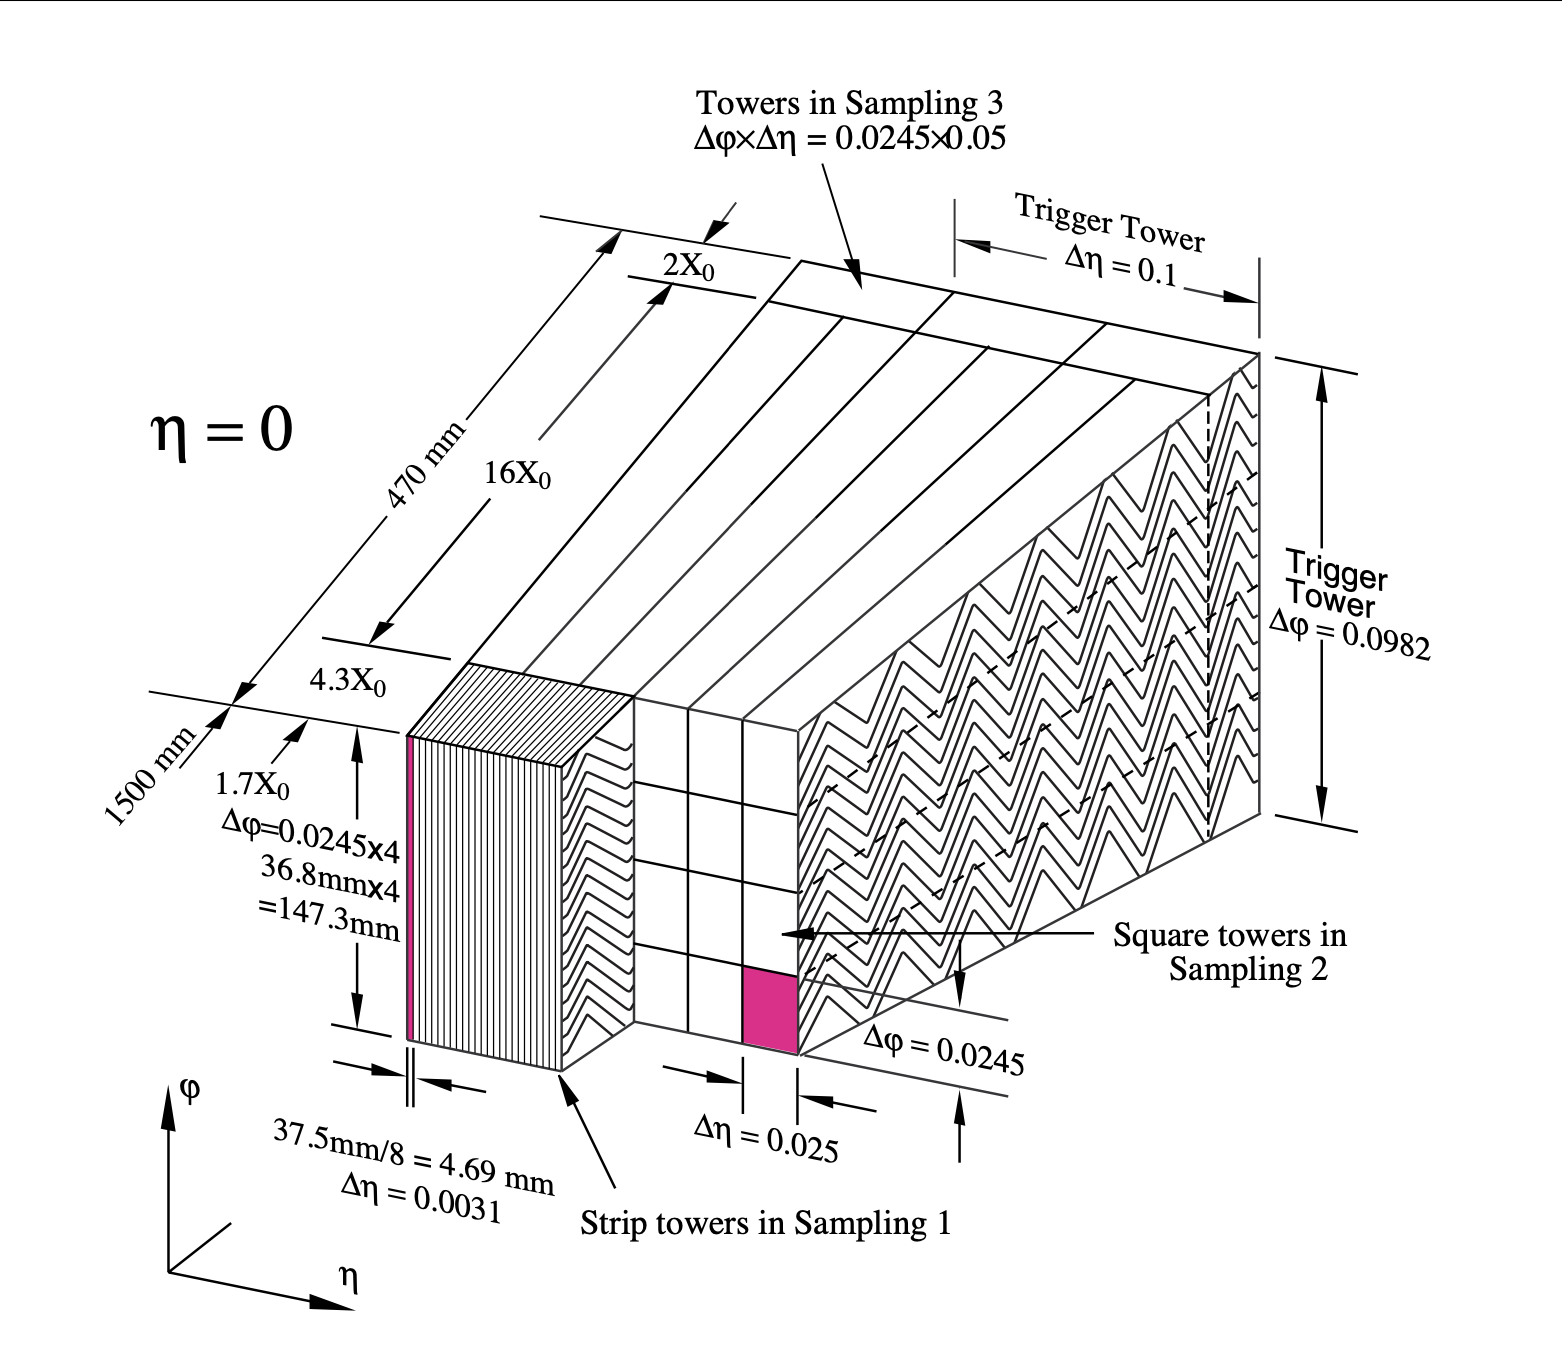
\includegraphics[width=0.6\textwidth]{figures/ch3/lar_accordion.png}
	\caption{Diagram of a segment of the EMB, demonstrating the accordion plate arrangement \cite{lar_tdr}}
	\label{fig:lar_accordion}
\end{figure}

% detection 
The detection principle for the LAr calorimeter is the current created by electrons which are released when a charged particle ionizes the liquid argon. In the barrel region, the electrons are driven towards the center electrodes by a 2000 V potential with a drift time of less than 450 ns \cite{lar_overview}. In the end-caps the voltage varies as a function of the radius in order to maintain a flat response \cite{lar_tdr}. The amount of current produced by the ionized electrons is proportional to the energy of the particle creating the signal. Figure \ref{fig:lar_pulse} shows the shape of the signal produced in the LAr calorimeter, before and after it undergoes shaping during the readout process. The shaping of the pulse enforces a positive peak and a negative tail, which ensures that subsequence pulses can be separated with the precision required for the 25 ns LHC bunch spacing \cite{lar_tdr}. \par

\begin{figure}
        \centering
	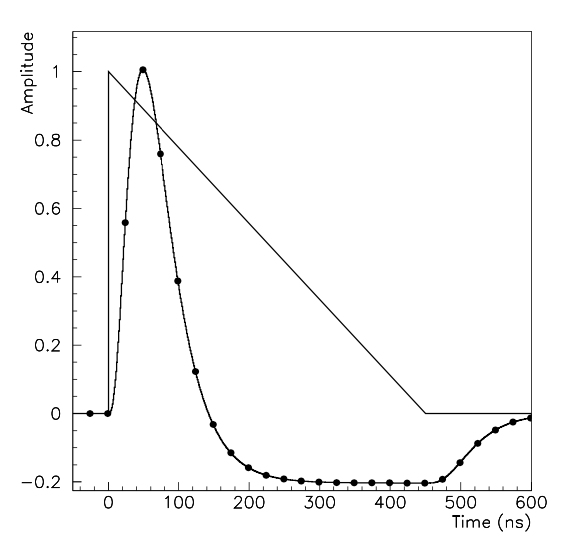
\includegraphics[width=0.5\textwidth]{figures/ch3/lar_pulse.png}
	\caption{A LAr pulse as produced in the detector (triangle) and after shaping (curve) \cite{lar_tdr}}
	\label{fig:lar_pulse}
\end{figure}

\subsubsection{Hadronic End-cap Calorimeter}
The HEC sits radially beyond the EMEC. The copper absorber plates in the HEC are oriented perpendicular to the beamline, with LAr as the active medium. Each end-cap is divided into two independent wheels; the inner wheel uses 25 mm copper plates, while the outer wheel uses 50 mm plates as a cost saving measure. In each wheel, the 8.5 mm plate gap is crossed by three parallel electrodes, creating and effective drift distance of 1.8 mm. This gap is illustrated in Figure \ref{fig:hec}. Each wheel is divided into 32 wedge-shaped modules, each containing their own set of readout electronics.\par

\begin{figure}
        \centering
	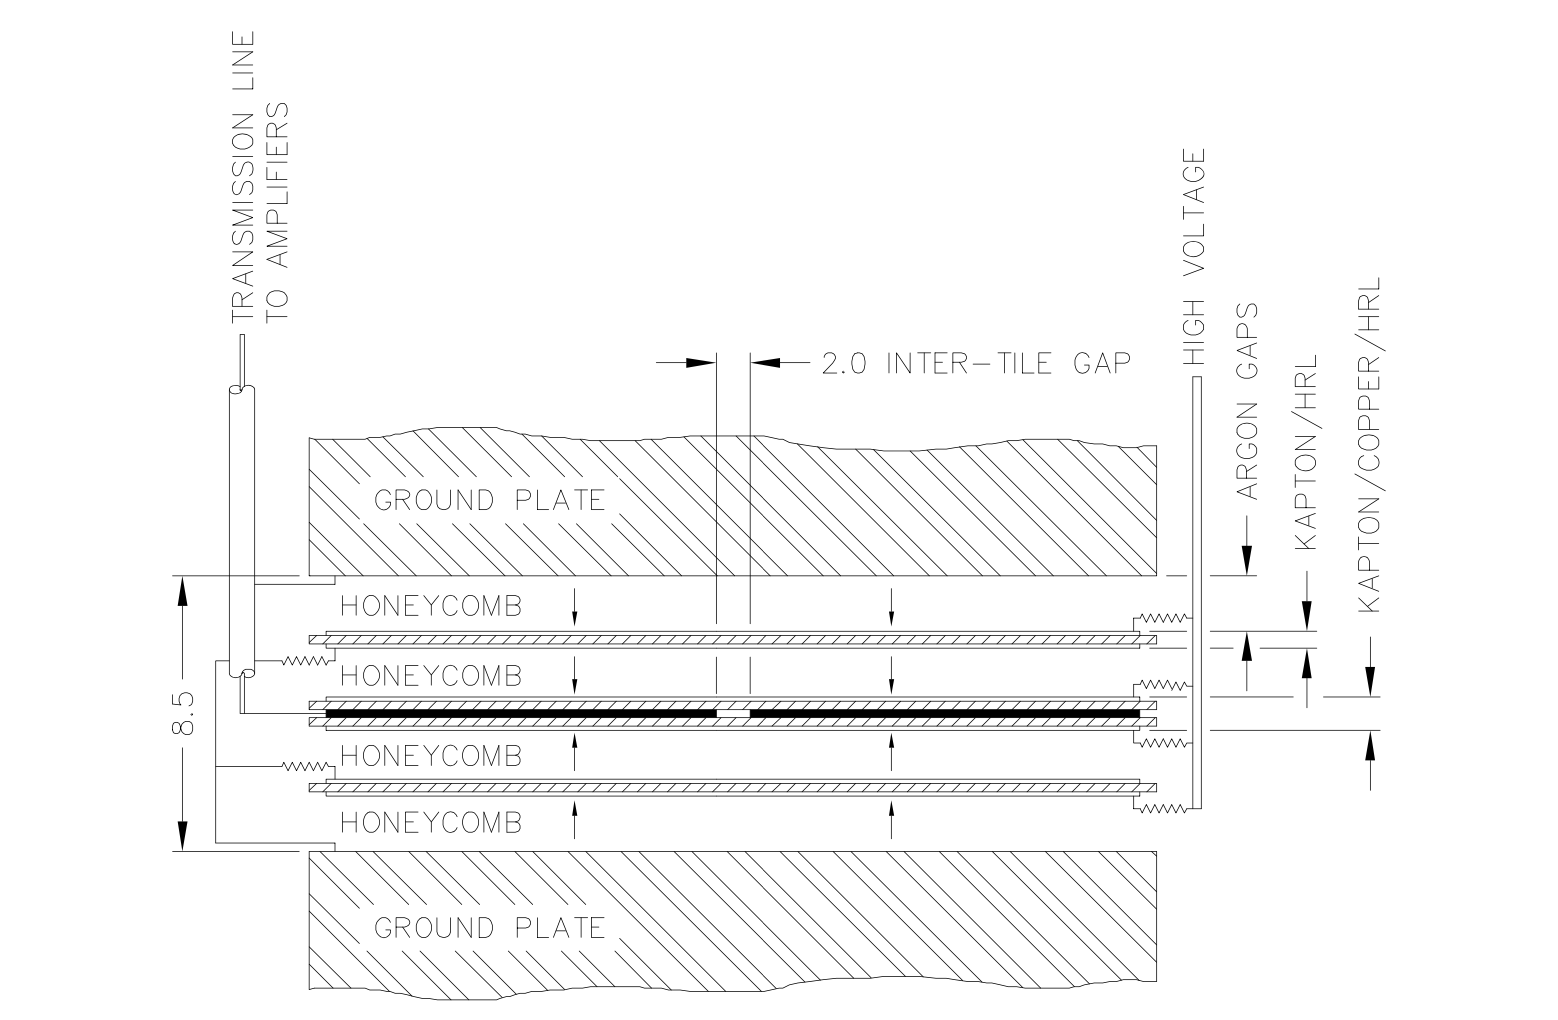
\includegraphics[width=0.5\textwidth]{figures/ch3/hec.png}
	\caption{Readout gap structure in HEC \cite{lar_tdr}}
	\label{fig:hec}
\end{figure}

\subsubsection{Forward Calorimeter}
The forward range is covered by the FCal, which provides both EM and hadronic calorimetry. It is composed of three active cylindrical modules; one EM module with copper absorber plates, and two hadronic modules with tungsten absorber plates. The plates are oriented perpendicular to the beamline, and LAr is used as the active material throughout. The electrodes of the FCal consist of tubes that run parallel to the beam line, arranged in a honeycomb pattern. The resulting LAr gaps are as small as 250 $\mu$m, which enables the FCal to handle the large influx of particles in the forward region \cite{lar_tdr}. 

\subsection{Tile Calorimeter}
The Tile Calorimeter (TileCal) provides hadronic calorimetry in the region $\eta < 1.7$, and surrounds the LAr calorimeter. It is responsible for measurements of jet energy and jet substructure, and also plays an important role in electron isolation and triggering (including muons) \cite{tile_tdr}. TileCal is composed of 3 sections, as shown in Figure \ref{fig:calorimeters}; a barrel calorimeter sits directly outside the LAr EMB and provides coverage up to $\eta < 1.0$. Two extended barrel sections sit outside the LAr endcaps and cover the region $0.8 < \eta < 1.7$. \par

TileCal is a sampling calorimeter composed of steel and plastic scintillator plates as illustrated in Figure \ref{fig:tileCal}. A total of 460,000 scintillators are read out by wavelength-shifting fibers. The fibers are gathered to define cells and in turn read out by photomultiplier tubes, which amplify the signal and convert it to an electrical signature. Each cell has an approximate granularity of $\Delta\eta \times \Delta\phi = 0.1 \times 0.1$. Each barrel is divided azimuthally into 64 independent modules, an example of which is show in Figure \ref{fig:tileCal}. The modules are each serviced by front-end electronic housed in a water-cooled drawer on the exterior of the module. \par

\begin{figure}
        \centering
	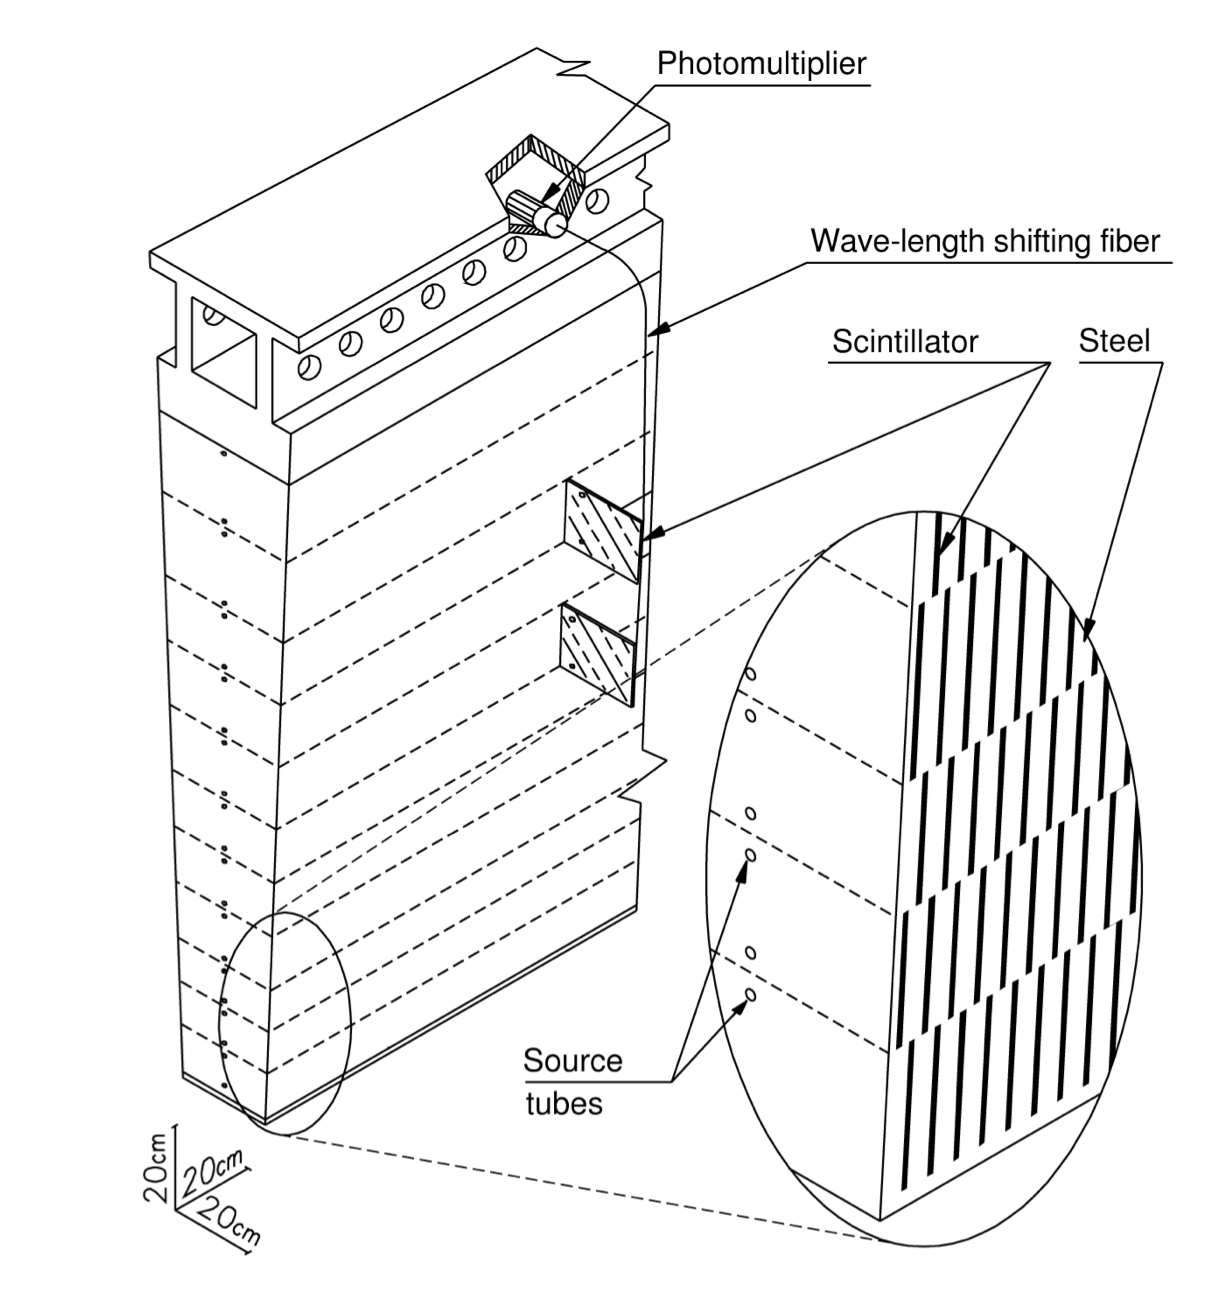
\includegraphics[width=0.5\textwidth]{figures/ch3/tileWedge.png}
	\caption{TileCal wedge module \cite{tile_tdr} }
	\label{fig:tileCal}
\end{figure}

The detection principle of the TileCal is the production of light from hadronic particles interacting with the scintillating tiles. When a hadronic particle hits the steel plate, a shower of particles are produced. The interaction of the shower with the plastic scintillator produces photons, the number and intensity of which are proportional to the original particle's energy. \\

\section{Muon Spectrometer}
Unlike electrons, photons, and hadrons, muons interact minimally with the ATLAS calorimeters, and can pass through large amounts of detector material without stopping. The ATLAS Muon Spectrometer (MS) provides additional tracking information to improve the identification and measurement of muons. The MS comprises the outermost layers of the detector, and is interspersed with toroid magnets (discussed in Section \ref{sec:magnets}), which provide a magnetic field of approximately 0.5 T. The magnetic field bends the trajectory of the muons as they pass through the detector, and the degree of the bend is directly correlated with the muon momentum. The path of the muon is primarily measured by hits in three layers of Monitored Drift Tube (MDT) precision chambers, which cover the range $|\eta|$ < 2.7. The barrel layout of the MS is show in Figure \ref{fig:muonSpec}. \par

\begin{figure}
        \centering
	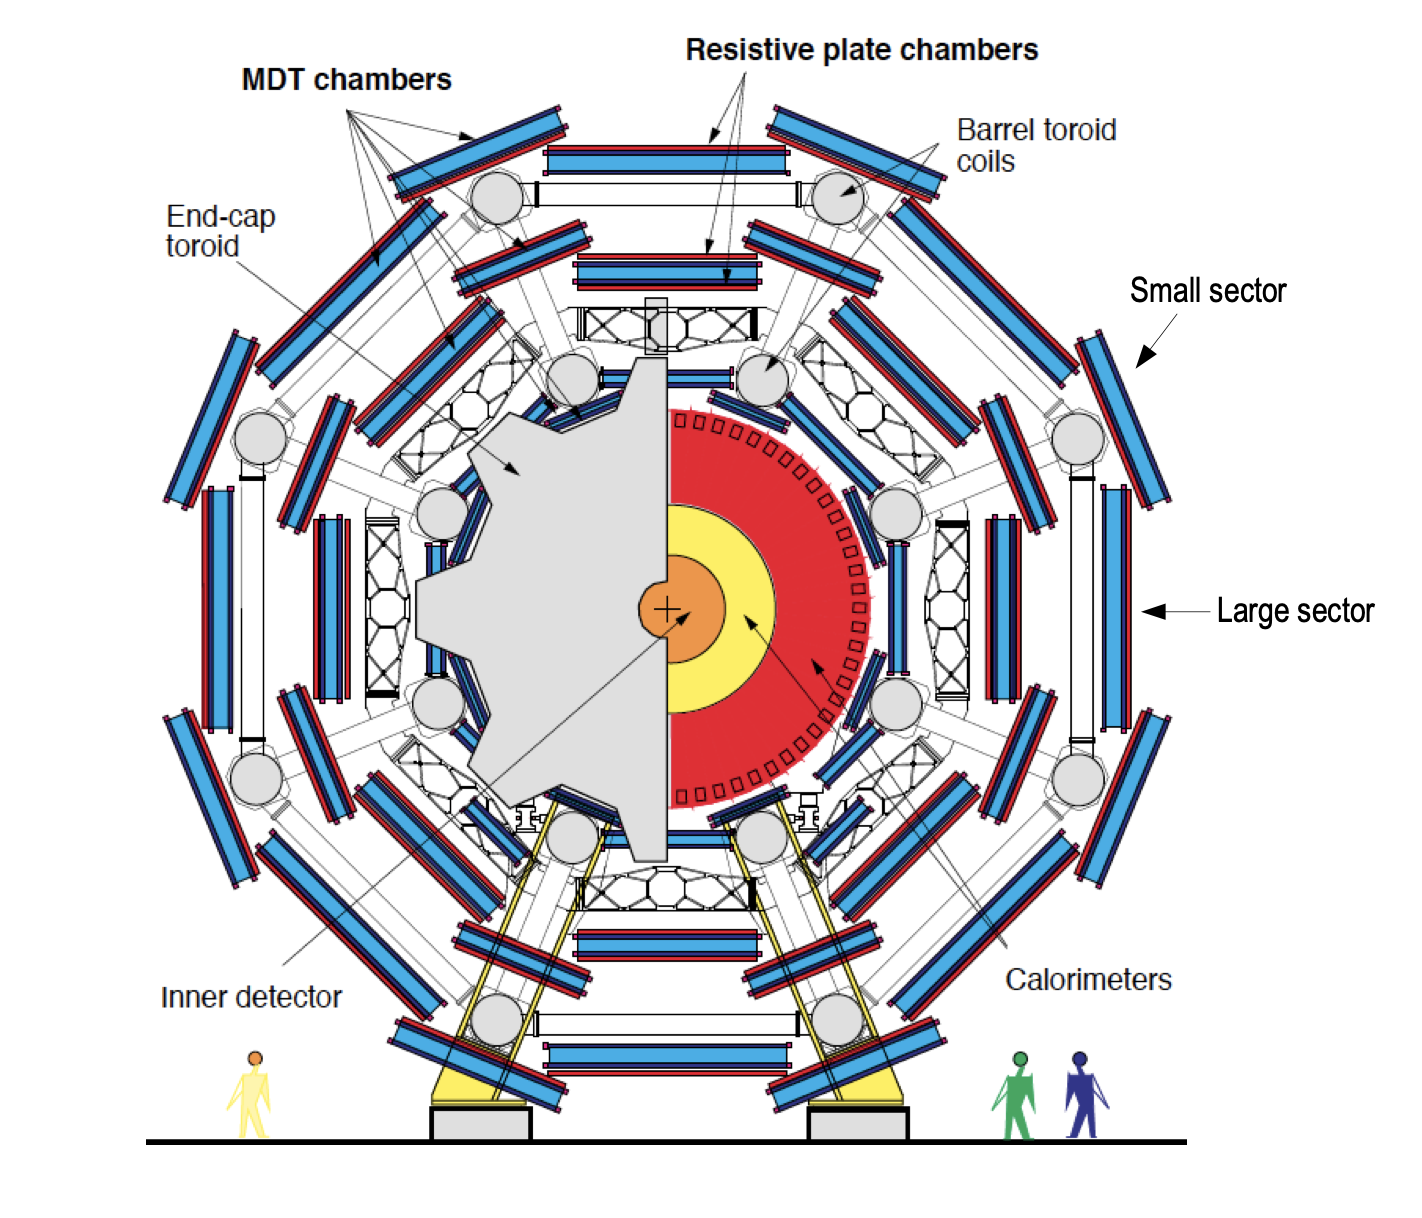
\includegraphics[width=0.7\textwidth]{figures/ch3/muonSpec.png}
	\caption{Cross section view of the muon spectrometer system \cite{muon_tdr} }
	\label{fig:muonSpec}
\end{figure}

Muon triggering is provided by three layers of Resistive Plate Chambers (RPC) in the barrel ($|\eta|$ < 1.05), and 3 - 4 layers of Thin Gap Chambers (TGC) in the end-caps (1.05 < $|\eta|$ < 2.4). RPCs and TGCs also provide muon track measurements in the non-bending coordinate ($\phi$). RPCs are constructed from two parallel resistive plates separated by a 2mm gap filled with a sensitive gas mixture. This provides a total of six independent measurements for each muon track, with a spatial resolution of $\sim$1 cm and a time resolution of $\sim$1 ns. Time measurements from the RPCs are primarily associated to hits in the MDT precision chambers to determine the bunch crossing. The time measurement is also used to reject cosmic muons, and to search for delayed signals. TCGs provide triggering in the end-cap regions, and consist of parallel 30 $\mu$m wires suspended in a sensitive gas mixture. TCGs provide high radiation tolerance and a fast response time, both features that are necessary for handling the high flux of muons in the forward region \cite{muon_tdr}.\par

Precision measurements of muon momentum and position are primarily achieved by MDTs. The MDTs are constructed from 30 mm diameter tubes, permeated by a gas mixture of 93\% Ar and 7\% CO\textsubscript{2}. The average single-tube spatial resolution is 80 $\mu$m. Each chamber consists of six drift tube layers, which together provide a muon track segment resolution of 35 $\mu$m. The momentum of the muons can be calculated from the bend in the muon trajectory as they pass through the 0.5T magnetic field provided by the toroids. For a $p_T$ = 1 TeV track, the average $p_T$ resolution is 11\%. In the inner most end-cap wheels, Cathode Strip Chambers (CSC) are used instead of MDTs, covering the region $2.0 < |\eta| < 2.7$. CSCs are multi-wire proportional chambers, with a cathode strip readout. The CSCs have a spatial resolution in the range of 50 $\mu$m, and a maximum drift time of about 30 ns, which makes them superior for handling the high flux of particles in the forward region \cite{muon_spec}. 

\section{Magnet System}
\label{sec:magnets}
The ATLAS magnet system consists of four sets of superconducting magnets: a barrel solenoid, a barrel toroid, and two end-cap toroids. The solenoid magnet produces a 2T magnetic field responsible for bending the trajectories of charged particles as they pass through the inner detector. The three toroid magnets provide a field of 0.5 - 1 T and curve the path of muons passing through the muon spectrometer.\par

The inner solenoid magnet is composed of over 9 km of niobium-titanium superconductor wires, which are imbedded into strengthen pure aluminum strips. The solenoid is just 4.5 cm thick, which minimizes interactions between the magnet material and particles passing through the detector. It is housed in the LAr cryostat, as described in section \ref{sec:lar}, which further reduces the amount of non-detector material required to support the solenoid. The return yoke of the magnet is provided by the iron absorber of the TileCal \cite{magnet_tdr}.\par

The central ATLAS toroid magnet, providing the magnetic field for the barrel region of the MS, is the largest toroidal magnet ever constructed at 25 m in length. The toroid is composed of eight individual coils, each housed in their own cryostat. The toroidal magnetic field is advantageous as the direction of the field is almost perpendicular to the path of the charged particles. 56 km of aluminum stabilized niobium-titanium-copper superconductor wire compose the magnet. In each end-cap, eight smaller superconducting coils extend the toroidal magnetic field to particles leaving the detector in the forward direction \cite{magnet_tdr}. Figure \ref{fig:magnets} shows the layout of the toroid magnets.

\begin{figure}
        \centering
	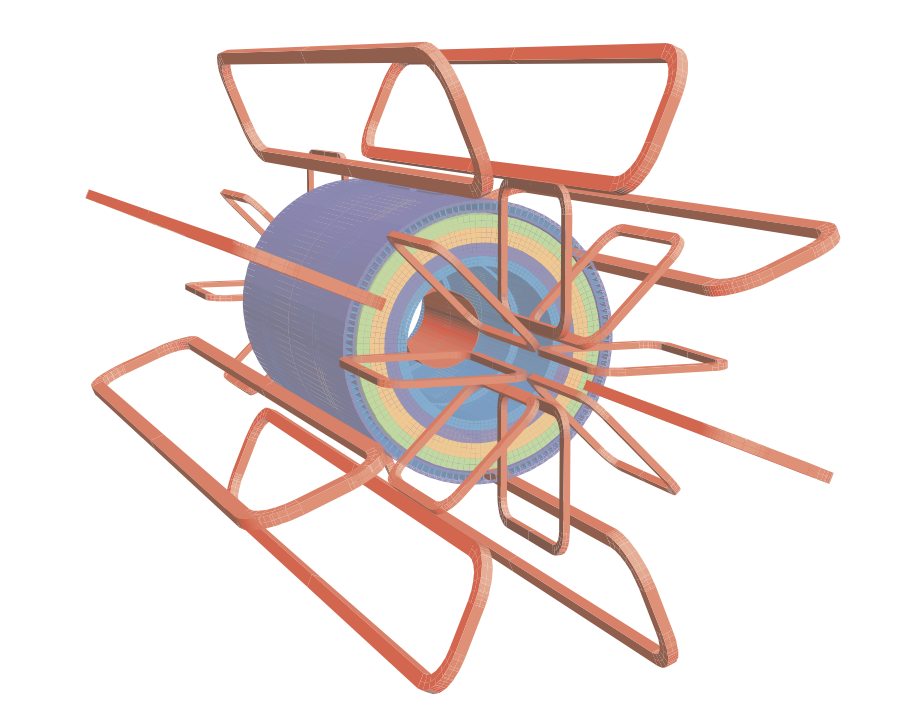
\includegraphics[width=0.65\textwidth]{figures/ch3/magnets.png}
	\caption{Layout of the barrel and endcap toroid magnets \cite{atlas_overview} }
	\label{fig:magnets}
\end{figure}

\section{Forward Detectors}
	In addition to the inner detector, calorimeters, and muon spectrometer, three smaller detectors provide coverage in the very forward region. The innermost forward detector, at 17 m from the interaction point, is the \textbf{LU}minosity measurement using \textbf{C}erenkov \textbf{I}ntegrating \textbf{D}etector (LUCID). LUCID's primary purpose is to measure the relative online-luminosity for the ATLAS detector, from inelastic $p-p$ scattering. The detector is composed of 20 aluminum Cerenkov tubes which surround the beam pipe and face towards the interaction point. \par
	The second forward detector is the Zero-Degree Calorimeter (ZDC), located 140 m from the interaction point in both directions, at the point where the LHC beam-pipe divides into two separate pipes. The ZDC's primary purpose is to detector forward neutrons from heavy ion collisions. \par
	The third forward detector is the Absolute Luminosity For ATLAS (ALFA) system, located 240 m from the interaction point in both directions. ALFA determines luminosity by measuring elastic scattering at small angles, from which luminosity can be calculated via the optical theorem. The detector is built from scintillating fiber trackers. These are connected to the accelerator vacuum via Roman pots, which allow the detector to come as close as 1mm to the beam without disrupting the machine vacuum. The LUCID and ALFA detectors are crucial to determining the real-time conditions of the beams and the total luminosity delivered to the ATLAS detector  \cite{atlas_overview}.

\section{Trigger and Data Acquisition}
	The trigger and Data Acquisition systems (TDAQ) are responsible for selecting the most viable events to save for further downstream processing. Because of the high luminosities delivered to the ATLAS detector, not all events recorded can be saved; the 40 MHz bunch crossing rate must be reduced by 5 orders of magnitude to an event storage rate of $\sim$1 kHz. The trigger system is composed of three distinct levels: Level 1 (L1), Level 2 (L2) and the event filter. Collectively the L2 trigger and the event filter form the High Level Trigger (HLT).\par

	The L1 trigger is implemented in the hardware of the ATLAS calorimeter and muon systems. The primary modality of the L1 trigger is to identify muons, electrons, photons, jets, and $\tau$-leptons with high transverse momentum. Particles with high transverse momentum are more likely to originate from direct, high energy collisions, which are most likely to produce interesting physics processes. The L1 trigger also identifies events with large missing transverse energy, which could be indicative of new physics. The L1 muon trigger (L1Muon) relies on RPC and TGC trigger chambers in the barrel and end-cap regions of the muon spectrometer. The L1 Calorimeter Trigger (L1Calo) uses reduced granularity information collected by all the calorimeter subsystems. Results from the L1Muon and L1Calo triggers are combined by the Central Trigger Processor (CTP), which implements a trigger `menu', listing various combinations of trigger requirements. The maximum L1 acceptance rate is 75 kHz, and the L1 trigger decision must reach the front-end electronics within 2.5 $\mu$s of it's associated bunch-crossing \cite{atlas_overview}.\par
	
	The L1 trigger defines a Region-of-Interest (RoI) for each passing event. The ROI is represented by the $\eta$-$\phi$ detector region where interesting features were identified by the L1 selection process. Information about the type of feature identified and the threshold which was exceeded to trigger the L1 response is also recorded. The ROI data is sent to the L2 trigger, which uses all of the available information within the ROI at full granularity and precision. The L2 trigger reduces the event rate from 75 kHz to 3.5 kHz, with an average processing time of 40 ms. The final stage of the HLT is the event filter, which reduces the event rate to 200 Hz. The event filter uses an offline analysis process to select fully rebuilt events which will be saved for further analysis. \par
	
	All levels of the ATLAS trigger system depend on specialized electronics. Each detector front-end system has a specialized Readout Driver (ROD) which collects information from several front-end data streams at once. The ROD is composed of front-end analogue processing, an L1 buffer which retains the information long enough for the L1 trigger decision, and dedicated links which send the front-end L1 triggered data to Data Acquisition System (DAQ). Any digital signals are formatted as raw data before being transferred to the DAQ.  The first stage of the DAQ temporarily stores the L1 data in local buffers. The ROI data is then requested by the L2 trigger, after which selected events are transferred to an event building system, before events passing the event filter are sent to the CERN computer center for permanent storage. The DAQ system not only allows for the readout of detector data, but is also responsible for the monitoring and configuration of the hardware and software components which make up the data readout system via the Detector Control System (DCS). \par
	
	The DCS allows centralized control of all detector subsystems simultaneously. It continually monitors operational conditions, reports any abnormal behavior to the operator, and can perform both automatic and manual interventions. The DCS reports on real time detector conditions such as high or low voltage detector electronics, gas and cooling systems, magnetic filed conditions, humidity and temperature. This information is continually monitored by experts in the ATLAS control room, so that action can be taken immediately to correct any issues that arise. The DCS also handles communication between detector systems, and other systems such as the LHC accelerator, the ATLAS magnets, and CERN technical services \cite{atlas_overview}. 

